\documentclass[../DoAn.tex]{subfiles}
\begin{document}

Chương~\ref{chap:de-xuat} đã đặc tả nhóm lệnh mở rộng phục vụ suy luận INT8 và cách ánh xạ nhóm lệnh này sang nhánh mô phỏng gem5. Tiếp nối phần thiết kế đó, chương này trình bày quá trình hiện thực, kiểm thử và đánh giá nhóm lệnh trong gem5 nhằm xác nhận ngữ nghĩa, kiểm tra hồi quy và phân tích xu hướng hiệu năng của các vòng lặp tính toán. Nội dung chương lần lượt mô tả các thành phần gem5 được bổ sung, bộ smoke test chức năng, thiết lập benchmark mô phỏng, kết quả thu được trên các cấu hình CPU/bộ nhớ và phần phân tích riêng cho mô hình vòng lặp phần cứng trong O3.

\section{Hiện thực nhóm lệnh mở rộng trong gem5}
\label{sec:hien-thuc-gem5}

Trên cơ sở đặc tả ở Chương~\ref{chap:de-xuat}, bước hiện thực trong gem5 đưa mỗi thao tác mở rộng vào đầy đủ đường đi của mô hình RISC-V, từ giải mã, tạo đối tượng lệnh, thực thi cho đến ghi nhận thống kê mô phỏng. Vì vậy, phần này tập trung vào các điểm tích hợp trong gem5: mã hóa thử nghiệm, ánh xạ từ mã lệnh sang định dạng hoặc lớp lệnh, và cơ chế cập nhật trạng thái khi lệnh được thực thi. Do ngữ nghĩa toán học của từng lệnh đã được trình bày ở Chương~\ref{chap:de-xuat}, nội dung dưới đây chỉ làm rõ những quyết định triển khai cần thiết để nhóm lệnh có thể chạy trong trình mô phỏng.

Như đã nêu ở Chương~\ref{chap:co-so-ly-thuyet}, gem5 sử dụng một ngôn ngữ đặc tả chuyên biệt cho ISA (ISA Domain-Specific Language, ISA DSL) để sinh đường giải mã, lớp lệnh và các đoạn C++ cần thiết cho mô hình thực thi \cite{gem5_docs_2026}. Hình~\ref{fig:gem5-ai-ext-implementation} tóm tắt luồng tích hợp được áp dụng trong đồ án. Trong luồng này, các tệp \texttt{decoder.isa}, \texttt{formats/*.isa} và \texttt{operands.isa} mô tả cách tách trường lệnh, lựa chọn định dạng và khai báo toán hạng. Từ các mô tả đó, trình xử lý ISA của gem5 sinh một phần mã C++; phần mã sinh ra tiếp tục được biên dịch cùng các lớp C++ bổ sung như \texttt{ai\_ext.hh}, \texttt{ai\_ext.cc} và các mở rộng của đường truy cập bộ nhớ. Nhờ vậy, bản gem5 sau khi biên dịch có thể giải mã các lệnh thử nghiệm và chạy các chương trình kiểm thử hoặc benchmark tương ứng.

\begin{figure}[H]
    \centering
    \begin{tikzpicture}[
    font=\scriptsize,
    block/.style={draw, rounded corners=2pt, align=center, minimum height=0.82cm, fill=gray!8},
    file/.style={block, text width=3.85cm, fill=cyan!8},
    proc/.style={block, text width=3.85cm, fill=yellow!15},
    cpp/.style={block, text width=3.85cm, fill=blue!8},
    outbox/.style={block, text width=3.85cm, fill=green!9},
    resultbox/.style={block, text width=3.85cm, fill=orange!12},
    side/.style={block, text width=3.05cm, fill=orange!12},
    note/.style={align=center, font=\scriptsize},
    arrow/.style={-{Latex[length=2mm]}, thick}
]
    \node[file] (dsl) at (0, 0) {Mô tả ISA\\\texttt{decoder.isa}\\\texttt{formats/*.isa}\\\texttt{operands.isa}};
    \node[proc] (parser) at (0, -1.85) {ISA parser\\sinh decoder\\và mã C++};
    \node[cpp] (cpp) at (0, -3.70) {C++ sinh ra\\và C++ bổ sung\\\texttt{ai\_ext.*}, \texttt{mem.*}};
    \node[proc] (compiler) at (0, -5.35) {Biên dịch gem5};
    \node[outbox] (bin) at (0, -6.95) {Tệp thực thi gem5\\chạy smoke test\\và benchmark};
    \node[resultbox] (stats) at (0, -8.55) {Kết quả mô phỏng\\và kiểm thử};

    \node[side] (decode) at (4.25, 0) {Phần đồ án bổ sung\\ánh xạ \texttt{custom-0}\\theo \texttt{funct3/funct7}};
    \node[side] (model) at (4.25, -3.70) {Mô hình hành vi\\lệnh số học,\\\texttt{PostIncLoad}\\và hardware loop};

    \draw[arrow] (dsl) -- (parser);
    \draw[arrow] (parser) -- (cpp);
    \draw[arrow] (cpp) -- (compiler);
    \draw[arrow] (compiler) -- (bin);
    \draw[arrow] (bin) -- (stats);

    \draw[arrow] (decode) -- (dsl);
    \draw[arrow] (model) -- (cpp);
\end{tikzpicture}

    \caption{Luồng hiện thực nhóm lệnh mở rộng trong gem5}
    \label{fig:gem5-ai-ext-implementation}
\end{figure}

Điểm vào của nhóm lệnh mở rộng nằm ở \texttt{decoder.isa}. Đồ án sử dụng vùng \texttt{custom-0} của RISC-V, tương ứng với mẫu \(\texttt{opcode[6:2]}=0x02\) và opcode đầy đủ \(\texttt{0x0B}\). Đoạn mã~\ref{lst:gem5-custom0-decode} trích phần ánh xạ chính trong \texttt{decoder.isa}. Ba lệnh dạng R gồm \texttt{mac}, \texttt{dot4\_acc} và \texttt{relu} dùng chung \(\texttt{funct3}=0\), sau đó được phân biệt bằng \texttt{funct7}; các thao tác còn lại được phân biệt bằng \texttt{funct3}. Cách tổ chức này gom toàn bộ mã hóa thử nghiệm trong một nhánh decode riêng và giữ nguyên đường giải mã của các lệnh chuẩn.

\begin{lstlisting}[
    basicstyle=\ttfamily\scriptsize,
    columns=fullflexible,
    keepspaces=true,
    frame=single,
    breaklines=true,
    caption={Ánh xạ vùng custom-0 trong decoder.isa},
    captionpos=b,
    label={lst:gem5-custom0-decode}
]
0x02: decode FUNCT3 {
    0x0: decode FUNCT7 {
        format MAC_R {
            0x00: mac();
        }
        format DOT4_ACC_R {
            0x01: dot4_acc();
        }
        format RELU_R {
            0x02: relu();
        }
    }
    format CLAMP_R {
        0x1: clamp();
    }
    format LP_SETUP_I {
        0x2: lp_setup();
    }
    format PostIncLoad {
        0x3: p_lw({{
            Rd_sd = Mem_sw;
            Rpw = rvSext(Rs1 + offset);
        }}, {{
            EA = rvSext(Rs1);
        }});
    }
}
\end{lstlisting}

Các tên \texttt{MAC\_R}, \texttt{DOT4\_ACC\_R}, \texttt{RELU\_R}, \texttt{CLAMP\_R} và \texttt{LP\_SETUP\_I} trong đoạn mã trên là các định dạng được liên kết với hàm khởi tạo của lớp lệnh tương ứng. Các liên kết này được khai báo trong \texttt{custom.isa}, còn phần thân của các lớp lệnh số học và \texttt{lp.setup} nằm trong \texttt{ai\_ext.hh} và \texttt{ai\_ext.cc}. Mỗi lớp lệnh khai báo tên hiển thị, danh sách toán hạng nguồn/đích và hàm \texttt{execute} để cập nhật trạng thái mô phỏng. Riêng với các lệnh tích lũy, \texttt{rd} được khai báo đồng thời là toán hạng nguồn và toán hạng đích, nhờ đó mô hình CPU vẫn quan sát đúng phụ thuộc dữ liệu của chuỗi cộng dồn.

Trường hợp \texttt{p.lw} thể hiện rõ vai trò của cơ chế định dạng và khuôn mẫu trong gem5. Trong đoạn mã~\ref{lst:gem5-custom0-decode}, phần \texttt{EA = rvSext(Rs1)} xác định địa chỉ tải bằng giá trị hiện tại của \texttt{rs1}, còn dòng \texttt{Rpw = rvSext(Rs1 + offset)} ghi lại con trỏ sau cập nhật. Để biểu diễn thao tác ghi lại \texttt{rs1}, đồ án bổ sung toán hạng \texttt{Rpw} trong \texttt{operands.isa}. Định dạng \texttt{PostIncLoad} trong \texttt{mem.isa} sau đó tái sử dụng đường load của gem5, nhưng thay đổi thứ tự tính địa chỉ và ghi kết quả phụ. Nhờ cách này, \texttt{p.lw} vẫn đi qua cơ chế truy cập bộ nhớ chuẩn của gem5, đồng thời biểu diễn được hiệu ứng hậu tăng địa chỉ.

Đối với \texttt{lp.setup}, phần decode chỉ lựa chọn lớp lệnh khởi tạo; hành vi đầy đủ của vòng lặp còn phụ thuộc vào các trạng thái điều khiển đi kèm. Đồ án bổ sung các misc-reg như \texttt{LPSTART}, \texttt{LPEND}, \texttt{LPCOUNT} và \texttt{LPACTIVE}, sau đó gắn logic vòng lặp vào hai hook cập nhật PC của ISA. Khi lệnh ở cuối vòng lặp được thực thi, \texttt{postAdvancePC} có thể đổi PC kế tiếp về \texttt{LPSTART}; khi lệnh cuối vòng lặp commit, \texttt{commitAdvancePC} cập nhật bộ đếm và trạng thái hoạt động của vòng lặp. Với O3, thời điểm công bố trạng thái vòng lặp và thời điểm khối lấy lệnh quan sát đường quay lại đầu vòng phức tạp hơn, nên phần này còn cần các điều chỉnh riêng ở execute, commit và khối lấy lệnh. Các điều chỉnh đó được phân tích riêng ở Mục~\ref{sec:phan-tich-hwloop-o3}.

Bảng~\ref{tab:gem5-ai-ext-components} hệ thống hóa các nhóm file và vai trò của chúng. Bảng này nhấn mạnh rằng phần gem5 của đồ án không chỉ là bộ test/benchmark, mà bao gồm cả các thay đổi ở tầng mô tả ISA, lớp lệnh, định dạng truy cập bộ nhớ, trạng thái phụ trợ và đường cập nhật PC.

\begin{table}[H]
    \centering
    \small
    \renewcommand{\arraystretch}{1.16}
    \begin{tabular}{|>{\raggedright\arraybackslash}p{3.45cm}|>{\raggedright\arraybackslash}p{9.45cm}|}
        \hline
        \textbf{Nhóm thành phần} & \textbf{Vai trò trong hiện thực gem5} \\
        \hline
        Giải mã và định dạng lệnh & \texttt{decoder.isa} nhận diện vùng \texttt{custom-0}; \texttt{custom.isa} ánh xạ các format như \texttt{MAC\_R}, \texttt{DOT4\_ACC\_R}, \texttt{CLAMP\_R} và \texttt{LP\_SETUP\_I} sang constructor của lớp lệnh. \\
        \hline
        Lớp lệnh số học và \texttt{lp.setup} & \texttt{ai\_ext.hh} và \texttt{ai\_ext.cc} khai báo lớp lệnh, danh sách toán hạng, hàm disassembly và hàm \texttt{execute}. \\
        \hline
        Tải hậu tăng & \texttt{mem.isa}, \texttt{mem.hh}, \texttt{mem.cc} và \texttt{operands.isa} bổ sung \texttt{PostIncLoad}, cách hiển thị \texttt{p.lw} và toán hạng \texttt{Rpw} để ghi lại con trỏ. \\
        \hline
        Trạng thái vòng lặp phần cứng & \texttt{regs/misc.hh} và \texttt{isa.cc} bổ sung các trạng thái \texttt{LPSTART}, \texttt{LPEND}, \texttt{LPCOUNT}, \texttt{LPACTIVE} và các điểm móc đổi hướng/cập nhật bộ đếm vòng lặp. \\
        \hline
        Hỗ trợ O3/khối lấy lệnh & Các đường execute, commit và khối lấy lệnh của O3 được bổ sung để xử lý thời điểm công bố trạng thái vòng lặp và giảm chi phí sửa PC ở backend. \\
        \hline
    \end{tabular}
    \caption{Các nhóm thay đổi chính trong gem5 cho nhóm lệnh mở rộng}
    \label{tab:gem5-ai-ext-components}
\end{table}

Từ các thành phần trên, phần hiện thực trong gem5 bám theo luồng mở rộng ISA của trình mô phỏng: bổ sung mã hóa trong ISA DSL, ánh xạ mã hóa tới lớp lệnh hoặc template phù hợp, rồi cập nhật các trạng thái mô phỏng liên quan. Sau khi các điểm tích hợp này được hoàn thiện, bộ kiểm thử chức năng được dùng để xác nhận rằng mô hình mới thực thi đúng các trường hợp quan trọng trước khi chuyển sang phân tích hiệu năng.

\section{Kiểm thử chức năng}
\label{sec:kiem-thu-chuc-nang-gem5}

Sau khi hoàn thiện các điểm tích hợp ở Mục~\ref{sec:hien-thuc-gem5}, bước kiểm thử đầu tiên là xác nhận ngữ nghĩa của từng lệnh ở mức chức năng. Bộ kiểm thử được tổ chức dưới dạng các chương trình smoke test chạy ở chế độ syscall emulation của gem5. Mỗi chương trình tự kiểm tra trạng thái thanh ghi, bộ nhớ hoặc luồng điều khiển sau khi thực thi lệnh mở rộng; nếu mọi điều kiện đều đúng, chương trình in ra chuỗi \texttt{PASS} tương ứng và thoát với mã trả về bằng 0. Trình kiểm thử của gem5 sau đó chạy chương trình trên các mô hình CPU đã chọn và dùng \texttt{MatchRegex} để xác nhận rằng đầu ra có đúng chuỗi \texttt{PASS}. Cách tổ chức này giúp tách rõ hai điều kiện: mô phỏng phải kết thúc thành công và kết quả quan sát được trong chương trình khách phải đúng với ngữ nghĩa mong đợi.

Bảng~\ref{tab:gem5-smoke-tests} tóm tắt phạm vi của ba nhóm smoke test. Hai nhóm \texttt{ai\_ops\_smoke} và \texttt{p\_lw\_smoke} được chạy trên \texttt{atomic} và \texttt{o3}, trong khi \texttt{hwloop\_smoke} được chạy thêm trên \texttt{minor} để kiểm tra đường cập nhật PC và cơ chế đổi hướng trên nhiều kiểu CPU hơn. Với \texttt{o3}, cấu hình kiểm thử sử dụng đường lấy lệnh mở rộng đã trình bày trong phần hiện thực; các chi tiết riêng của vòng lặp phần cứng trên O3 được phân tích sâu hơn ở Mục~\ref{sec:phan-tich-hwloop-o3}.

\begin{table}[H]
    \centering
    \small
    \setlength{\tabcolsep}{3pt}
    \renewcommand{\arraystretch}{1.18}
    \begin{tabular}{|>{\raggedright\arraybackslash}p{3.30cm}|>{\raggedright\arraybackslash}p{4.95cm}|>{\raggedright\arraybackslash}p{2.20cm}|>{\raggedright\arraybackslash}p{1.55cm}|}
        \hline
        \textbf{Nhóm kiểm thử} & \textbf{Nội dung xác nhận chính} & \textbf{Mô hình CPU} & \textbf{Kết quả} \\
        \hline
        \texttt{ai\_ops\_smoke} & Kiểm tra \texttt{mac}, \texttt{dot4\_acc}, \texttt{relu}, \texttt{clamp}; bao gồm hành vi với \texttt{x0} và chặn trên của \texttt{clamp} đọc từ thanh ghi. & \texttt{atomic}, \texttt{o3} & Đạt \\
        \hline
        \texttt{p\_lw\_smoke} & Kiểm tra lệnh tải trước khi cập nhật địa chỉ, hậu tăng \texttt{rs1} bằng \(\mathrm{sext}(\mathrm{imm12})\), trường hợp \texttt{rd=x0} và hằng dịch âm. & \texttt{atomic}, \texttt{o3} & Đạt \\
        \hline
        \texttt{hwloop\_smoke} & Kiểm tra cơ chế đổi hướng của \texttt{lp.setup}, nhánh số vòng lặp bằng 0 và giá trị immediate thô theo quy ước CORE-V. & \texttt{atomic}, \texttt{minor}, \texttt{o3} & Đạt \\
        \hline
    \end{tabular}
    \caption{Phạm vi kiểm thử chức năng cho nhóm lệnh mở rộng trong gem5}
    \label{tab:gem5-smoke-tests}
\end{table}

Để làm rõ cách các kiểm thử này xác nhận ngữ nghĩa mà không cần quan sát trực tiếp trạng thái bên trong gem5, có thể xét trường hợp đại diện của \texttt{p\_lw\_smoke}. Chương trình đặt hai từ dữ liệu liên tiếp trong bộ nhớ, thực hiện lệnh \texttt{p.lw}, rồi so sánh đồng thời giá trị được nạp vào thanh ghi đích và giá trị mới của thanh ghi cơ sở. Trường hợp này xác nhận thứ tự thực hiện của lệnh là đọc dữ liệu tại địa chỉ ban đầu của \texttt{rs1} trước, sau đó mới cập nhật \texttt{rs1} theo \(\mathrm{sext}(\mathrm{imm12})\). Kiểm thử cũng bao gồm trường hợp \texttt{rd=x0} để bảo đảm việc bỏ qua ghi vào thanh ghi đích không làm mất tác động cập nhật thanh ghi cơ sở. Các nhóm kiểm thử còn lại được tổ chức theo cùng nguyên tắc: mỗi điều kiện quan trọng được chuyển thành một phép so sánh trực tiếp trong chương trình khách trước khi in ra chuỗi \texttt{PASS}.

Bộ kiểm thử được chạy bằng lệnh trong Đoạn mã~\ref{lst:gem5-smoke-command}. Tùy chọn \texttt{--skip-build} được dùng khi bản gem5 cần kiểm tra đã được biên dịch trước đó, nhờ vậy lần chạy này chỉ tập trung vào kiểm thử hồi quy của các chương trình smoke test.

\begin{lstlisting}[
    basicstyle=\ttfamily\scriptsize,
    columns=fullflexible,
    keepspaces=true,
    frame=single,
    breaklines=true,
    caption={Lệnh chạy bộ smoke test cho nhóm lệnh mở rộng},
    captionpos=b,
    label={lst:gem5-smoke-command}
]
cd /home/duydonv/gem5/tests
./main.py run gem5/riscv_ai_ext --length=quick --skip-build
\end{lstlisting}

Kết quả thu được là \texttt{14 Passed}. Con số này gồm bảy lần chạy mô phỏng và bảy bước kiểm tra \texttt{MatchRegex} tương ứng với chuỗi \texttt{PASS} của từng chương trình. Cụ thể, \texttt{ai\_ops\_smoke} và \texttt{p\_lw\_smoke} mỗi nhóm tạo bốn mục kiểm thử trong testlib, còn \texttt{hwloop\_smoke} tạo sáu mục do được chạy trên ba mô hình CPU. Việc toàn bộ các mục kiểm thử đều đạt cho thấy phần giải mã, lớp lệnh, truy cập bộ nhớ hậu tăng và trạng thái vòng lặp phần cứng đã nhất quán ở mức chức năng trước khi chuyển sang các benchmark hiệu năng ở các mục tiếp theo.

\section{Thiết lập benchmark mô phỏng}
\label{sec:thiet-lap-benchmark-gem5}

Sau khi các lệnh mở rộng đã vượt qua kiểm thử chức năng, bước tiếp theo là xây dựng các benchmark nhỏ để quan sát tác động của từng nhóm lệnh trong điều kiện mô phỏng có kiểm soát. Các benchmark không nhằm mô phỏng trọn vẹn một mô hình AI hoàn chỉnh, mà cô lập những mẫu tính toán đại diện đã xuất hiện trong Chương~3: nhân--cộng tích lũy, tích vô hướng int8 đóng gói, chặn miền giá trị và giảm chi phí điều khiển trong vòng lặp.

Mỗi chương trình benchmark được tổ chức thành ba phần. Trước hết, dữ liệu đầu vào được khởi tạo ngoài vùng đo để chi phí sinh dữ liệu không lẫn vào kết quả. Ngay trước khi đi vào vùng nhân tính toán, chương trình gọi \texttt{m5\_reset\_stats}; ngay sau khi vùng nhân kết thúc, chương trình gọi \texttt{m5\_dump\_reset\_stats}. Trình tổng hợp kết quả đọc phần thống kê đầu tiên trong \texttt{stats.txt}, do đó các chỉ số được báo cáo chỉ phản ánh vùng nhân thay vì bao gồm khởi động chương trình, in kết quả hoặc thoát tiến trình. Sau vùng đo, chương trình in ra dòng \texttt{BENCH\_RESULT} kèm giá trị kiểm tra; giá trị này được dùng để xác nhận rằng các biến thể scalar và custom tạo cùng kết quả số học.

Bảng~\ref{tab:gem5-benchmark-cases} trình bày ba ca chạy được dùng cho mỗi benchmark. Ca thứ nhất là mốc scalar trên cây gem5 chưa mở rộng. Ca thứ hai chạy lại cùng mã scalar trên cây gem5 đã chỉnh sửa, nhờ đó có thể phát hiện phần chênh lệch do thay đổi mô hình mô phỏng thay vì do lệnh mới. Ca thứ ba mới là bản dùng lệnh mở rộng và được so sánh với mốc scalar để tính mức tăng tốc.

\begin{table}[H]
    \centering
    \small
    \setlength{\tabcolsep}{4pt}
    \renewcommand{\arraystretch}{1.18}
    \begin{tabular}{|>{\raggedright\arraybackslash}p{3.15cm}|>{\raggedright\arraybackslash}p{3.35cm}|>{\raggedright\arraybackslash}p{5.60cm}|}
        \hline
        \textbf{Ca chạy} & \textbf{Tệp thực thi gem5} & \textbf{Vai trò trong so sánh} \\
        \hline
        \texttt{baseline}\newline\texttt{\_scalar} & \texttt{gem5\_baseline} & Chạy chương trình scalar làm mốc hiệu năng ban đầu. \\
        \hline
        \texttt{update}\newline\texttt{\_scalar} & gem5 đã mở rộng & Chạy lại cùng chương trình scalar để kiểm tra phần chênh lệch do thay đổi mô hình gem5. \\
        \hline
        \texttt{update}\newline\texttt{\_custom} & gem5 đã mở rộng & Chạy chương trình dùng lệnh mở rộng; kết quả được đối chiếu với mốc scalar bằng chu kỳ mô phỏng và giá trị kiểm tra. \\
        \hline
    \end{tabular}
    \caption{Ba ca chạy trong mỗi benchmark mô phỏng}
    \label{tab:gem5-benchmark-cases}
\end{table}

Ba nhóm benchmark trong Bảng~\ref{tab:gem5-benchmark-groups} được chọn để tăng dần mức độ sử dụng phần mở rộng. Nhóm \texttt{mac\_clamp} kiểm tra riêng lợi ích của phép nhân--cộng tích lũy và chặn miền giá trị. Nhóm \texttt{dot4\_acc\_clamp} giữ nguyên cách tải dữ liệu và điều khiển vòng lặp, chỉ thay phần tích vô hướng bốn lane int8 bằng \texttt{dot4\_acc}. Nhóm \texttt{dot4\_plw\_lp\_clamp} bổ sung thêm \texttt{p.lw} và \texttt{lp.setup}, nên phản ánh trường hợp tối ưu hơn cho luồng dữ liệu tuần tự.

\begin{table}[H]
    \centering
    \small
    \setlength{\tabcolsep}{3pt}
    \renewcommand{\arraystretch}{1.18}
    \begin{tabular}{|>{\raggedright\arraybackslash}p{3.35cm}|>{\raggedright\arraybackslash}p{3.20cm}|>{\raggedright\arraybackslash}p{2.85cm}|>{\raggedright\arraybackslash}p{3.65cm}|}
        \hline
        \textbf{Benchmark} & \textbf{Mục tiêu đo} & \textbf{Kích thước vùng nhân} & \textbf{Thao tác mở rộng trong bản custom} \\
        \hline
        \texttt{mac\_clamp} & Nhân--cộng tích lũy và chặn trên kết quả. & \(512 \times 32 = 16\,384\) lần MAC. & Dùng \texttt{mac} cho tích lũy và \texttt{clamp} với chặn trên đọc từ thanh ghi. \\
        \hline
        \texttt{dot4\_acc}\newline\texttt{\_clamp} & Tích vô hướng int8 đóng gói, chưa thay đổi đường tải và điều khiển vòng lặp. & \(128 \times 64 = 8\,192\) bước dot4, tương ứng \(32\,768\) phép nhân int8 theo lane. & Dùng \texttt{dot4\_acc} cho mỗi từ đóng gói và \texttt{clamp} ở cuối mỗi đầu ra. \\
        \hline
        \texttt{dot4\_plw}\newline\texttt{\_lp\_clamp} & Tích vô hướng int8 đóng gói kết hợp tải hậu tăng và vòng lặp phần cứng. & \(128 \times 64 = 8\,192\) bước dot4, cùng kích thước với nhóm trên. & Dùng \texttt{lp.setup} cho vòng trong, hai lệnh \texttt{p.lw} để nạp dữ liệu tuần tự, sau đó \texttt{dot4\_acc} và \texttt{clamp}. \\
        \hline
    \end{tabular}
    \caption{Các nhóm benchmark dùng trong đánh giá mô phỏng gem5}
    \label{tab:gem5-benchmark-groups}
\end{table}

Các benchmark được chạy bằng \texttt{run\_perf\_compare.py}. Mặc định, chương trình này sử dụng mô hình CPU \texttt{o3}, bảng mạch \texttt{SimpleBoard} ở tần số 3~GHz, bộ nhớ \texttt{DDR3\_1600} và phân cấp bộ nhớ đệm gồm L1I 32~KiB, L1D 32~KiB và L2 dùng chung 256~KiB. Với CPU \texttt{o3}, cấu hình này bật đường lấy lệnh tách rời và bộ dự đoán nhánh LTAGE để mô hình hóa đường lấy lệnh có hỗ trợ cập nhật mục tiêu cho vòng lặp phần cứng. Ngoài cấu hình có cache mặc định, hai điểm nhạy cảm bộ nhớ cũng được dùng: \texttt{--no-cache} để nối trực tiếp CPU tới DDR3 và \texttt{--no-cache --memory fast-ram} để xấp xỉ vùng RAM cục bộ có độ trễ thấp. Các lệnh chạy tương ứng được tóm tắt trong Đoạn mã~\ref{lst:gem5-perf-command}.

\begin{lstlisting}[
    basicstyle=\ttfamily\scriptsize,
    columns=fullflexible,
    keepspaces=true,
    frame=single,
    breaklines=true,
    caption={Các lệnh chạy benchmark theo ba điểm cấu hình chính},
    captionpos=b,
    label={lst:gem5-perf-command}
]
python3 tests/gem5/riscv_ai_ext/run_perf_compare.py --skip-build
python3 tests/gem5/riscv_ai_ext/run_perf_compare.py --skip-build --no-cache
python3 tests/gem5/riscv_ai_ext/run_perf_compare.py --skip-build --no-cache --memory fast-ram
\end{lstlisting}

Như vậy, các ca chạy trong benchmark được giữ thống nhất về vùng đo, cấu hình mô phỏng và cách ghi thống kê. Phần tiếp theo trình bày cách trích lọc các trường cần thiết từ đầu ra của gem5 và phân tích xu hướng hiệu năng thu được.

\section{Kết quả mô phỏng và phân tích xu hướng}
\label{sec:ket-qua-mo-phong-gem5}
\raggedbottom

Nguồn số liệu của mục này là phần thống kê vùng đo trong \texttt{stats.txt} do gem5 sinh ra sau khi chạy benchmark. Hình~\ref{fig:gem5-stats-txt-excerpt} minh họa một trích đoạn rút gọn của tệp thống kê này. Trong đầu ra thô, các trường phục vụ so sánh như số lệnh mô phỏng và số chu kỳ xuất hiện cùng nhiều thống kê khác của gem5, nên đồ án cần trích lọc đúng các trường thuộc phần thống kê đầu tiên tương ứng với vùng nhân đã được khoanh bằng m5ops trước khi lập bảng kết quả.

\begin{figure}[H]
    \centering
    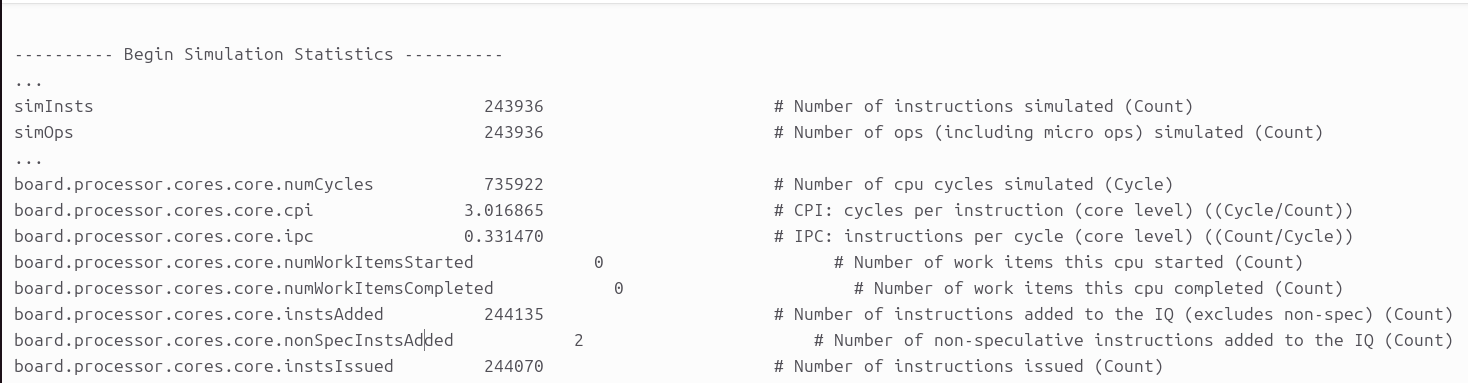
\includegraphics[width=0.98\textwidth]{Hinh_ve/gem5_stats_txt_excerpt.png}
    \caption{Ví dụ trích đoạn đầu ra thống kê thô trong tệp \texttt{stats.txt} của gem5}
    \label{fig:gem5-stats-txt-excerpt}
\end{figure}
\afterpage{\flushbottom}

Quy trình trích lọc trên được áp dụng cho ba cấu hình tương ứng với các lệnh chạy ở Đoạn mã~\ref{lst:gem5-perf-command}: O3 có cache, NoCache DDR3 và NoCache fast-ram. Trước khi đưa số liệu vào so sánh, giá trị kiểm tra của \texttt{baseline\_scalar}, \texttt{update\_scalar} và \texttt{update\_custom} đều được đối chiếu và cho kết quả khớp nhau. Ngoài ra, số chu kỳ của \texttt{update\_scalar} trùng với \texttt{baseline\_scalar}, cho thấy các thay đổi trong gem5 không làm lệch đường scalar dùng làm mốc.

Trên cơ sở các lần chạy đã được trích lọc và đối chiếu nhất quán, Bảng~\ref{tab:gem5-perf-results} tổng hợp số chu kỳ mô phỏng và số lệnh động trong vùng nhân của hai bản scalar và custom, cùng mức tăng tốc so với mốc scalar. Các giá trị tăng tốc được tính theo công thức \(S = C_{\text{scalar}} / C_{\text{custom}}\), trong đó \(C\) là số chu kỳ được trích từ lần ghi thống kê ngay sau vùng nhân. Các chỉ số gắn trực tiếp với cơ chế vòng lặp phần cứng, như đổi hướng PC, tra cứu BTB và dự đoán nhánh, được tách sang Mục~\ref{sec:phan-tich-hwloop-o3} để phần này tập trung vào xu hướng hiệu năng chung của các kernel.

\begin{table}[H]
    \centering
    \footnotesize
    \setlength{\tabcolsep}{2.5pt}
    \renewcommand{\arraystretch}{1.18}
    \begin{tabular}{|>{\raggedright\arraybackslash}p{2.20cm}|>{\raggedright\arraybackslash}p{2.10cm}|>{\raggedleft\arraybackslash}p{1.85cm}|>{\raggedleft\arraybackslash}p{1.85cm}|>{\raggedleft\arraybackslash}p{1.85cm}|>{\raggedleft\arraybackslash}p{1.85cm}|>{\centering\arraybackslash}p{1.45cm}|}
        \hline
        \textbf{Benchmark} & \textbf{Cấu hình} & \textbf{Chu kỳ scalar} & \textbf{Chu kỳ custom} & \textbf{Lệnh động scalar} & \textbf{Lệnh động custom} & \textbf{Tăng tốc} \\
        \hline
        \multirow{3}{*}{\texttt{mac\_clamp}} & O3 có cache & \(55\,613\) & \(56\,446\) & \(243\,936\) & \(226\,328\) & \(0{,}9852\times\) \\
        \cline{2-7}
        & NoCache DDR3 & \(7\,049\,770\) & \(7\,032\,875\) & \(243\,936\) & \(226\,328\) & \(1{,}0024\times\) \\
        \cline{2-7}
        & NoCache fast-ram & \(735\,922\) & \(735\,403\) & \(243\,936\) & \(226\,328\) & \(1{,}0007\times\) \\
        \hline
        \multirow{3}{*}{\shortstack[l]{\texttt{dot4\_acc}\\\texttt{\_clamp}}} & O3 có cache & \(83\,297\) & \(28\,452\) & \(298\,781\) & \(60\,701\) & \(2{,}9276\times\) \\
        \cline{2-7}
        & NoCache DDR3 & \(11\,092\,838\) & \(3\,405\,261\) & \(298\,781\) & \(60\,701\) & \(3{,}2576\times\) \\
        \cline{2-7}
        & NoCache fast-ram & \(1\,158\,007\) & \(356\,031\) & \(298\,781\) & \(60\,701\) & \(3{,}2525\times\) \\
        \hline
        \multirow{3}{*}{\shortstack[l]{\texttt{dot4\_plw}\\\texttt{\_lp\_clamp}}} & O3 có cache & \(83\,297\) & \(29\,214\) & \(298\,781\) & \(28\,189\) & \(2{,}8513\times\) \\
        \cline{2-7}
        & NoCache DDR3 & \(11\,092\,838\) & \(1\,151\,329\) & \(298\,781\) & \(28\,189\) & \(9{,}6348\times\) \\
        \cline{2-7}
        & NoCache fast-ram & \(1\,158\,007\) & \(133\,651\) & \(298\,781\) & \(28\,189\) & \(8{,}6644\times\) \\
        \hline
    \end{tabular}
    \caption{Kết quả mô phỏng các benchmark trên ba cấu hình gem5}
    \label{tab:gem5-perf-results}
\end{table}

Để nhìn rõ hơn xu hướng giữa các nhóm lệnh, Hình~\ref{fig:gem5-perf-speedup} biểu diễn lại cột tăng tốc của Bảng~\ref{tab:gem5-perf-results}. Bảng số liệu cho phép đối chiếu chi tiết giữa chu kỳ và số lệnh động, trong khi hình này nhấn mạnh ba xu hướng chính: \texttt{mac\_clamp} gần như không cải thiện, \texttt{dot4\_acc\_clamp} tăng tốc ổn định quanh mức \(3\times\), còn \texttt{dot4\_plw\_lp\_clamp} phụ thuộc mạnh hơn vào cấu hình bộ nhớ.

\begin{figure}[H]
    \centering
    \resizebox{0.95\textwidth}{!}{\begin{tikzpicture}[
    x=1cm,
    y=0.39cm,
    font=\scriptsize,
    axis/.style={black!75, thick},
    gridline/.style={black!15, thin},
    cached/.style={fill=blue!55!black},
    ddr/.style={fill=green!50!black},
    fast/.style={fill=orange!80!black},
    legend/.style={anchor=west, align=left},
    value/.style={font=\tiny, anchor=south}
]
    \draw[axis] (0,0) -- (10.2,0);
    \draw[axis] (0,0) -- (0,10.55);

    \foreach \y/\lab in {0/{0},2/{2},4/{4},6/{6},8/{8},10/{10}} {
        \draw[gridline] (0,\y) -- (10.0,\y);
        \draw[axis] (-0.06,\y) -- (0.06,\y);
        \node[anchor=east] at (-0.14,\y) {\lab};
    }

    \node[rotate=90, anchor=south] at (-0.9,5.25) {Tăng tốc so với scalar};

    \draw[cached] (0.70,0) rectangle (1.12,0.99);
    \draw[ddr]    (1.20,0) rectangle (1.62,1.00);
    \draw[fast]   (1.70,0) rectangle (2.12,1.00);

    \draw[cached] (3.80,0) rectangle (4.22,2.93);
    \draw[ddr]    (4.30,0) rectangle (4.72,3.26);
    \draw[fast]   (4.80,0) rectangle (5.22,3.25);

    \draw[cached] (6.90,0) rectangle (7.32,2.85);
    \draw[ddr]    (7.40,0) rectangle (7.82,9.63);
    \draw[fast]   (7.90,0) rectangle (8.32,8.66);

    \node[value] at (0.91,1.13) {0.99};
    \node[value] at (1.41,1.14) {1.00};
    \node[value] at (1.91,1.14) {1.00};
    \node[value] at (4.01,3.07) {2.93};
    \node[value] at (4.51,3.40) {3.26};
    \node[value] at (5.01,3.39) {3.25};
    \node[value] at (7.11,2.99) {2.85};
    \node[value] at (7.61,9.77) {9.63};
    \node[value] at (8.11,8.80) {8.66};

    \node[align=center, anchor=north] at (1.41,-0.35) {\texttt{mac}\\\texttt{clamp}};
    \node[align=center, anchor=north] at (4.51,-0.35) {\texttt{dot4\_acc}\\\texttt{clamp}};
    \node[align=center, anchor=north] at (7.61,-0.35) {\texttt{dot4\_plw}\\\texttt{lp\_clamp}};

    \draw[cached] (8.75,6.85) rectangle (9.00,7.20);
    \node[legend] at (9.10,7.03) {O3 có cache};
    \draw[ddr] (8.75,6.10) rectangle (9.00,6.45);
    \node[legend] at (9.10,6.28) {NoCache DDR3};
    \draw[fast] (8.75,5.35) rectangle (9.00,5.70);
    \node[legend] at (9.10,5.53) {NoCache fast-ram};
\end{tikzpicture}
}
    \caption{Xu hướng tăng tốc của các benchmark trong mô phỏng gem5}
    \label{fig:gem5-perf-speedup}
\end{figure}

Với \texttt{mac\_clamp}, bản custom gần như không nhanh hơn bản scalar. Trong cấu hình O3 có cache, bản custom còn chậm hơn nhẹ, đạt \(0{,}9852\times\). Kết quả này cho thấy không phải mọi phép gộp lệnh đều trực tiếp chuyển thành tăng tốc theo chu kỳ. Ở benchmark này, lệnh \texttt{mac} thay thế cặp nhân--cộng scalar nhưng vẫn tích lũy qua cùng một thanh ghi đích, do đó chuỗi phụ thuộc dữ liệu theo từng bước lặp không thay đổi đáng kể. Trong khi đó, O3 có khả năng lập lịch chồng lấp một phần các phép nhân, cộng và tải dữ liệu của bản scalar. Vì vậy, mặc dù số lệnh động giảm từ \(243\,936\) xuống \(226\,328\), tức khoảng \(7{,}2\%\), phần giảm này chưa đủ để tạo lợi ích rõ rệt về chu kỳ. Ở hai cấu hình NoCache, chi phí truy cập bộ nhớ và lấy lệnh chi phối nhiều hơn, khiến chênh lệch giữa hai bản chỉ dao động quanh \(1\times\).

Với \texttt{dot4\_acc\_clamp}, mức tăng tốc rõ ràng hơn, từ \(2{,}9276\times\) đến \(3{,}2576\times\). Đây là kết quả phù hợp với mục tiêu của lệnh \texttt{dot4\_acc}: bốn phép nhân int8 theo lane và các phép cộng tương ứng trong bản scalar được gom vào một lệnh tích vô hướng đóng gói. Số lệnh động trong cấu hình O3 có cache giảm từ \(298\,781\) xuống \(60\,701\), tương đương giảm gần \(80\%\). Tuy nhiên, mức tăng tốc theo chu kỳ chỉ xấp xỉ \(3\times\) vì vùng nhân không chỉ gồm phép nhân--cộng. Chương trình vẫn phải tải dữ liệu, cập nhật chỉ số vòng lặp, kiểm tra điều kiện lặp và thực hiện \texttt{clamp} ở cuối mỗi đầu ra. Nói cách khác, \texttt{dot4\_acc} rút gọn phần tính toán cốt lõi của tích vô hướng, nhưng các chi phí phụ trợ quanh vòng lặp vẫn đặt giới hạn cho mức tăng tốc toàn kernel.

Với \texttt{dot4\_plw\_lp\_clamp}, kết quả phụ thuộc mạnh vào cấu hình bộ nhớ. Benchmark này không chỉ dùng \texttt{dot4\_acc}, mà còn thay các cập nhật con trỏ tường minh bằng \texttt{p.lw} và thay nhánh vòng lặp bằng \texttt{lp.setup}. Vì vậy, số lệnh động giảm sâu hơn, từ \(298\,781\) xuống \(28\,189\), tức hơn \(90\%\). Sau khi tối ưu đường cập nhật vòng lặp phần cứng, cấu hình O3 có cache đạt \(2{,}8513\times\), tiệm cận hơn với \texttt{dot4\_acc\_clamp} nhưng vẫn thấp hơn nhẹ. Nguyên nhân là khi cache che bớt chi phí lấy lệnh và truy cập dữ liệu, lợi ích từ việc rút gọn thân vòng lặp không còn biểu hiện toàn bộ ở số chu kỳ; ngoài ra mô hình vòng lặp phần cứng trong O3 vẫn có chi phí cập nhật luồng lấy lệnh. Ngược lại, ở hai cấu hình NoCache, bản custom đạt \(9{,}6348\times\) với DDR3 và \(8{,}6644\times\) với fast-ram. Khi không có cache, mỗi lệnh được lấy và mỗi truy cập dữ liệu đều đi qua mô hình bộ nhớ, nên việc giảm mạnh số lệnh trong thân vòng lặp tạo ra tác động lớn hơn. Sự khác biệt giữa DDR3 và fast-ram cũng cho thấy nhóm này nhạy với giả thiết về độ trễ bộ nhớ. Do đó, các con số NoCache không được dùng như dự đoán định lượng trực tiếp cho phần cứng thật, nhưng vẫn cho thấy xu hướng nhất quán: khi chi phí lấy lệnh và truy cập bộ nhớ tăng, việc rút gọn thân vòng lặp bằng nhóm lệnh mở rộng đem lại lợi ích rõ rệt hơn.

\section{Phân tích mô hình vòng lặp phần cứng trong O3}
\label{sec:phan-tich-hwloop-o3}

Kết quả ở Mục~\ref{sec:ket-qua-mo-phong-gem5} cho thấy \texttt{dot4\_plw\_lp\_clamp} giảm rất mạnh số lệnh động, nhưng mức tăng tốc trong O3 có cache không tăng tương ứng với mức giảm số lệnh. Nguyên nhân cần được phân tích riêng vì \texttt{lp.setup} không phải là một nhánh thông thường. Lệnh này thiết lập các trạng thái \texttt{LPSTART}, \texttt{LPEND}, \texttt{LPCOUNT} và \texttt{LPACTIVE}; khi một lệnh ở cuối vòng lặp được thực thi tại \texttt{LPEND}, PC kế tiếp có thể được đổi về \texttt{LPSTART} nếu bộ đếm vòng lặp vẫn còn lớn hơn một. Trong mô hình O3, việc này phức tạp hơn so với mô hình in-order vì khối lấy lệnh, execute và commit không quan sát trạng thái vòng lặp tại cùng một thời điểm.

Hình~\ref{fig:hwloop-o3-frontend} trình bày lưu đồ xử lý vòng lặp phần cứng trong mô hình O3 của gem5. Lưu đồ này tách ba điểm quyết định chính: lệnh hiện tại đã chạm \texttt{LPEND} hay chưa, khối lấy lệnh có dự đoán được mục tiêu \texttt{LPSTART} kịp thời hay không, và sau commit thì \texttt{LPCOUNT} còn hay đã hết. Ở đường xử lý thuận lợi, sau khi \texttt{lp.setup} công bố trạng thái vòng lặp, BAC/FTQ có thể xem \texttt{LPEND} như một điểm đổi hướng xác định và đưa luồng lấy lệnh về \texttt{LPSTART} sớm. Nếu thông tin này chưa kịp xuất hiện ở khối lấy lệnh, lệnh cuối vòng lặp vẫn đi tới execute; khi đó backend phải sửa PC và thống kê \texttt{nonControlRedirects} tăng lên. Sau khi lệnh cuối vòng commit, bộ đếm \texttt{LPCOUNT} được cập nhật; nếu vòng lặp còn tiếp tục thì mục tiêu \texttt{LPSTART} được duy trì, ngược lại trạng thái vòng lặp được xóa.

\begin{figure}[H]
    \centering
    \begin{tikzpicture}[
    font=\small,
    node distance=0.58cm and 0.92cm,
    terminator/.style={
        draw,
        rounded corners=9pt,
        align=center,
        minimum height=0.78cm,
        text width=2.95cm,
        fill=blue!6
    },
    process/.style={
        draw,
        rectangle,
        align=center,
        minimum height=0.78cm,
        text width=3.05cm,
        fill=green!7
    },
    warn/.style={
        draw,
        rectangle,
        align=center,
        minimum height=0.78cm,
        text width=3.05cm,
        fill=orange!10
    },
    decision/.style={
        draw,
        diamond,
        aspect=2.15,
        align=center,
        inner xsep=1pt,
        inner ysep=1pt,
        text width=2.35cm,
        fill=yellow!12
    },
    arrow/.style={-{Latex[length=2mm]}, thick}
]
    \node[terminator] (setup) {Bắt đầu\\\texttt{lp.setup}};
    \node[process, below=of setup] (regs) {Cập nhật\\\texttt{LPSTART}, \texttt{LPEND}\\\texttt{LPCOUNT}, \texttt{LPACTIVE}};
    \node[process, below=of regs] (body) {Thân vòng\\\texttt{LPSTART} \(\ldots\) \texttt{LPEND}};
    \node[decision, below=of body] (tail) {Chạm\\\texttt{LPEND}?};
    \node[decision, below=of tail] (predict) {Front-end\\dự đoán kịp?};
    \node[process, right=of predict] (frontend) {BAC/FTQ\\đưa fetch về\\\texttt{LPSTART}};
    \node[warn, below=of predict] (backend) {IEW sửa PC\\\texttt{nonControl}\\\texttt{Redirects}};
    \node[process, below=of backend] (commit) {Commit lệnh cuối\\giảm \texttt{LPCOUNT}\\và cập nhật BTB};
    \node[decision, below=of commit] (check) {Sau commit\\\texttt{LPCOUNT}\\còn?};
    \node[process, below left=0.70cm and 0.70cm of check] (again) {Giữ mục tiêu\\\texttt{LPSTART}};
    \node[terminator, below right=0.70cm and 0.70cm of check] (done) {Kết thúc vòng\\xóa mục tiêu\\tắt \texttt{LPACTIVE}};

    \draw[arrow] (setup) -- (regs);
    \draw[arrow] (regs) -- (body);
    \draw[arrow] (body) -- (tail);
    \draw[arrow] (tail) -- node[right] {có} (predict);
    \draw[arrow] (tail.west) -- ++(-0.80,0) node[pos=0.15, above] {chưa} |- (body.west);
    \draw[arrow] (predict) -- node[above] {có} (frontend);
    \draw[arrow] (frontend) |- (commit.east);
    \draw[arrow] (predict) -- node[right] {không} (backend);
    \draw[arrow] (backend) -- (commit);
    \draw[arrow] (commit) -- (check);
    \draw[arrow] (check) -| node[pos=0.28, above] {có} (again.north);
    \draw[arrow] (check) -| node[pos=0.28, above] {không} (done.north);
    \draw[arrow] (again.west) -- ++(-0.75,0) |- (body.west);
\end{tikzpicture}

    \caption{Lưu đồ xử lý vòng lặp phần cứng trong mô hình O3 của gem5}
    \label{fig:hwloop-o3-frontend}
\end{figure}

Để tách chi phí điều khiển vòng lặp khỏi phần tính toán của benchmark chính, đồ án sử dụng một microbenchmark riêng gồm ba biến thể. Biến thể \texttt{ref} thực hiện cùng khối tính toán nhưng mở cuộn hoàn toàn 32 lần, do đó không còn cạnh quay lại đầu vòng trong thân vòng trong. Biến thể \texttt{swloop} dùng nhánh phần mềm \texttt{bnez}. Biến thể \texttt{hwloop} dùng \texttt{lp.setup} với thân vòng gồm 8 lệnh không nén và số vòng lặp trong là 32. Ba quy mô \texttt{small}, \texttt{medium} và \texttt{large} chỉ thay đổi số lần lặp ngoài, lần lượt là \(1\,024\), \(4\,096\) và \(16\,384\). Vì mỗi lần thiết lập vòng trong có \(32-1\) lần quay lại đầu vòng, số lần quay lại đầu vòng về mặt logic của biến thể \texttt{hwloop} bằng \(\text{outer\_repeats} \times 31\).

Bảng~\ref{tab:hwloop-o3-microbench} trình bày kết quả microbenchmark trên cấu hình O3 có cache. Cột sửa PC ở backend, tương ứng với thống kê \texttt{nonControlRedirects}, cho biết số lần backend vẫn phải sửa PC cho một lệnh không phải nhánh điều khiển thông thường; cột tỷ lệ xử lý sớm biểu thị phần các lần quay lại đầu vòng đã được khối lấy lệnh xử lý trước khi cần sửa PC ở execute. Trong hai cột chu kỳ và lệnh động, giá trị trước và sau dấu ``/'' lần lượt ứng với \texttt{swloop} và \texttt{hwloop}.

\begin{table}[H]
    \centering
    \small
    \setlength{\tabcolsep}{2pt}
    \renewcommand{\arraystretch}{1.18}
    \begin{tabular*}{\textwidth}{@{\extracolsep{\fill}}|>{\raggedright\arraybackslash}p{1.52cm}|>{\raggedleft\arraybackslash}p{1.10cm}|>{\raggedleft\arraybackslash}p{1.32cm}|>{\raggedleft\arraybackslash}p{1.37cm}|>{\raggedleft\arraybackslash}p{1.32cm}|>{\raggedleft\arraybackslash}p{1.80cm}|>{\raggedleft\arraybackslash}p{2.03cm}|>{\centering\arraybackslash}p{1.49cm}|}
        \hline
        \textbf{Quy mô} & \textbf{Lặp ngoài} & \textbf{Lần quay lại} & \textbf{Sửa PC backend} & \textbf{Tỷ lệ xử lý sớm} & \textbf{Chu kỳ}\newline\textbf{sw/hw} & \textbf{Lệnh động}\newline\textbf{sw/hw} & \textbf{Tăng tốc}\newline\textbf{so với sw} \\
        \hline
        \texttt{small} & \(1\,024\) & \(31\,744\) & \(1\,024\) & \(96{,}77\%\) & \(150\,346/\)\newline\(235\,128\) & \(426\,401/\)\newline\(360\,865\) & \(0{,}6394\times\) \\
        \hline
        \texttt{medium} & \(4\,096\) & \(126\,976\) & \(4\,096\) & \(96{,}77\%\) & \(595\,786/\)\newline\(936\,339\) & \(1\,704\,360/\)\newline\(1\,442\,216\) & \(0{,}6363\times\) \\
        \hline
        \texttt{large} & \(16\,384\) & \(507\,904\) & \(16\,384\) & \(96{,}77\%\) & \(2\,361\,171/\)\newline\(3\,737\,207\) & \(6\,816\,161/\)\newline\(5\,767\,585\) & \(0{,}6318\times\) \\
        \hline
    \end{tabular*}
    \caption{Microbenchmark vòng lặp phần cứng trên O3 có cache}
    \label{tab:hwloop-o3-microbench}
\end{table}

Kết quả trong Bảng~\ref{tab:hwloop-o3-microbench} cho thấy đường lấy lệnh đã xử lý sớm phần lớn các lần quay lại đầu vòng lặp: chỉ còn \(1/31\) số lần quay lại của mỗi lần thiết lập vòng trong đi tới backend dưới dạng \texttt{nonControlRedirects}. Biến thể \texttt{hwloop} cũng giảm số lệnh động so với \texttt{swloop}; ở quy mô \texttt{large}, số lệnh giảm từ \(6\,816\,161\) xuống \(5\,767\,585\), tương đương khoảng \(15{,}4\%\). Tuy nhiên, trong cấu hình O3 có cache, biến thể \texttt{hwloop} vẫn chậm hơn \texttt{swloop}. Điều này cho thấy chi phí còn lại của các lần sửa PC ở backend là đáng kể khi phần lấy lệnh và truy cập dữ liệu đã được cache che bớt. Với quy mô \texttt{large}, \texttt{hwloop} tăng thêm \(1\,373\,781\) chu kỳ so với biến thể mở cuộn \texttt{ref}; nếu chia cho \(16\,384\) lần sửa PC còn lại, chi phí trung bình xấp xỉ 84 chu kỳ cho mỗi lần sửa. Đây là lý do ở Mục~\ref{sec:ket-qua-mo-phong-gem5}, bản \texttt{dot4\_plw\_lp\_clamp} trong O3 có cache không vượt \texttt{dot4\_acc\_clamp} dù số lệnh động giảm sâu hơn.

Khi bỏ cache, xu hướng thuận lợi hơn cho vòng lặp phần cứng. Với quy mô \texttt{large}, cấu hình NoCache DDR3 đạt \(1{,}3928\times\) so với \texttt{swloop} và không còn \texttt{nonControlRedirects}; cấu hình NoCache fast-ram đạt \(1{,}3696\times\) dù vẫn còn \(16\,384\) lần sửa PC ở backend. Các kết quả này phù hợp với phân tích ở Mục~\ref{sec:ket-qua-mo-phong-gem5}: khi chi phí lấy lệnh và truy cập bộ nhớ trở nên đáng kể, việc loại bỏ nhánh phần mềm và rút gọn thân vòng lặp tạo ra lợi ích rõ hơn. Ngược lại, trong O3 có cache, lợi ích của \texttt{lp.setup} bị giới hạn bởi chi phí đồng bộ giữa trạng thái vòng lặp và khối lấy lệnh. Vì vậy, mô hình hiện tại được dùng để giải thích xu hướng và chỉ ra điểm còn nhạy của O3, thay vì quy toàn bộ lợi ích của \texttt{lp.setup} về số lệnh động.

Chương này đã trình bày quá trình đưa nhóm lệnh mở rộng vào gem5, kiểm thử chức năng và đánh giá xu hướng hiệu năng qua các benchmark mô phỏng. Phần hiện thực cho thấy nhóm lệnh được tích hợp từ mức mô tả ISA, lớp lệnh, truy cập bộ nhớ hậu tăng cho đến trạng thái vòng lặp phần cứng; bộ smoke test xác nhận các ngữ nghĩa chính đều hoạt động đúng trên các mô hình CPU được chọn. Các benchmark cho thấy lợi ích của nhóm lệnh phụ thuộc vào loại thao tác được thay thế: \texttt{mac\_clamp} gần như không cải thiện trên O3, \texttt{dot4\_acc\_clamp} thể hiện lợi ích ổn định của tích vô hướng int8 đóng gói, còn \texttt{dot4\_plw\_lp\_clamp} cho thấy lợi ích lớn hơn khi chi phí lấy lệnh và truy cập bộ nhớ trở nên đáng kể. Phần phân tích riêng về O3 cũng chỉ ra rằng \texttt{lp.setup} không chỉ là vấn đề ngữ nghĩa ISA, mà còn phụ thuộc vào thời điểm khối lấy lệnh quan sát được trạng thái vòng lặp. Vì mô phỏng gem5 trong chương này sử dụng mã hóa thử nghiệm và mô hình O3 không trùng với CV32E40P trên kit DE2i-150, các số liệu thu được không được dùng như dự đoán chu kỳ trực tiếp cho phần cứng thật; vai trò chính của chúng là kiểm chứng thiết kế ở mức mô hình và làm rõ những xu hướng hiệu năng cần được đối chiếu. Chương~\ref{chap:thuc-nghiem} tiếp tục thực hiện bước đối chiếu này thông qua kết quả chạy trên kit thực nghiệm.


\end{document}
